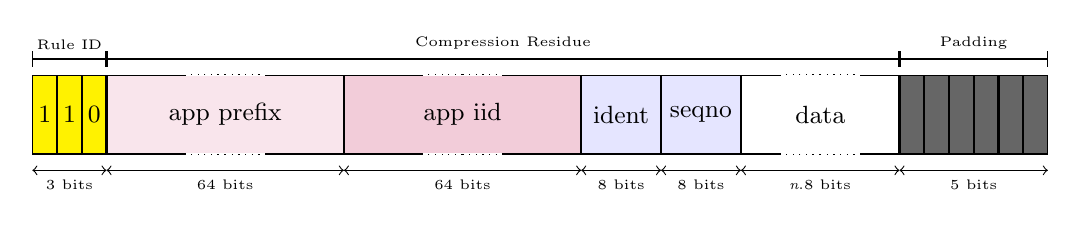
\begin{tikzpicture}

\draw (0,0) node (b1)  [rectangle, draw, minimum height=1cm, minimum width = 0.3cm, fill=yellow] {};
\draw(b1) node {\small{1}};
\draw (b1.east) node (b2)  [right, rectangle, draw, minimum height=1cm, minimum width = 0.3cm, fill=yellow] {};
\draw(b2) node {\small{1}};
\draw (b2.east) node (b3)  [right,rectangle, draw, minimum height=1cm, minimum width = 0.3cm, fill=yellow] {};
\draw(b3) node {\small{0}};

\path(b1.north) -- +(0, 0.2) coordinate(hlineu);

\draw [|-|] (b1.west |- hlineu) -- coordinate(a) (b3.east |- hlineu) ;
\draw (a) node [above] {\tiny{Rule ID}};

\path(b1.south) -- +(0, -0.2) coordinate(hline);

\draw [<->] (b1.west |- hline) -- coordinate(a) (b3.east |- hline) ;
\draw (a) node [below] {\tiny{3 bits}};


\draw (b3.east) node (pref) [right, rectangle, draw, minimum height=1cm, minimum width=3cm, fill=purple!10]{};

\draw [white, thick] (pref.north) -- +(0.5, 0);
\draw [white, thick] (pref.north) -- +(-0.5, 0);
\draw [dotted] (pref.north) -- +(0.5, 0);
\draw [dotted] (pref.north) -- +(-0.5, 0);

\draw [white, thick] (pref.south) -- +(0.5, 0);
\draw [white, thick] (pref.south) -- +(-0.5, 0);
\draw [dotted] (pref.south) -- +(0.5, 0);
\draw [dotted] (pref.south) -- +(-0.5, 0);

\draw (pref) node {\small{app prefix}};

\path(b1.south) -- +(0, -0.2) coordinate(hline);


\draw (pref.east) node (iid) [right, rectangle, draw, minimum height=1cm, minimum width=3cm, fill=purple!20]{};

\draw [white, thick] (iid.north) -- +(0.5, 0);
\draw [white, thick] (iid.north) -- +(-0.5, 0);
\draw [dotted] (iid.north) -- +(0.5, 0);
\draw [dotted] (iid.north) -- +(-0.5, 0);

\draw [white, thick] (iid.south) -- +(0.5, 0);
\draw [white, thick] (iid.south) -- +(-0.5, 0);
\draw [dotted] (iid.south) -- +(0.5, 0);
\draw [dotted] (iid.south) -- +(-0.5, 0);

\draw (iid) node {\small{app iid}};

\path(b1.south) -- +(0, -0.2) coordinate(hline);

\draw [<->] (pref.west |- hline) -- coordinate(a) (pref.east |- hline) ;
\draw (a) node [below] {\tiny{64 bits}};

\draw [<->] (iid.west |- hline) -- coordinate(a) (iid.east |- hline) ;
\draw (a) node [below] {\tiny{64 bits}};

\draw (iid.east) node (ident) [right, rectangle, draw, minimum height=1cm, minimum width=1cm, fill=blue!10]{};
\draw (ident.text) node {\small{ident}};

\draw [<->] (ident.west |- hline) -- coordinate(a) (ident.east |- hline) ;
\draw (a) node [below] {\tiny{8 bits}};

\draw (ident.east) node (seqno) [right, rectangle, draw, minimum height=1cm, minimum width=1cm, fill=blue!10]{};
\draw (seqno.text) node {\small{seqno}};

\draw [<->] (seqno.west |- hline) -- coordinate(a) (seqno.east |- hline) ;
\draw (a) node [below] {\tiny{8 bits}};

\draw (seqno.east) node (data) [right, rectangle, draw, minimum height=1cm, minimum width=2cm]{};
\draw (data.text) node {\small{data}};

\draw [white, thick] (data.north) -- +(0.5, 0);
\draw [white, thick] (data.north) -- +(-0.5, 0);
\draw [dotted] (data.north) -- +(0.5, 0);
\draw [dotted] (data.north) -- +(-0.5, 0);

\draw [white, thick] (data.south) -- +(0.5, 0);
\draw [white, thick] (data.south) -- +(-0.5, 0);
\draw [dotted] (data.south) -- +(0.5, 0);
\draw [dotted] (data.south) -- +(-0.5, 0);

\draw [<->] (data.west |- hline) -- coordinate(a) (data.east |- hline) ;
\draw (a) node [below] {\tiny{\textit{n}.8 bits}};

\draw (data.east) node (p1)  [right, rectangle, draw, minimum height=1cm, minimum width = 0.3cm, fill=black!60] {};
\draw (p1.east) node (p2)  [right, rectangle, draw, minimum height=1cm, minimum width = 0.3cm, fill=black!60] {};
\draw (p2.east) node (p3)  [right,rectangle, draw, minimum height=1cm, minimum width = 0.3cm, fill=black!60] {};
\draw (p3.east) node (p4)  [right,rectangle, draw, minimum height=1cm, minimum width = 0.3cm, fill=black!60] {};
\draw (p4.east) node (p5)  [right,rectangle, draw, minimum height=1cm, minimum width = 0.3cm, fill=black!60] {};
\draw (p5.east) node (p6)  [right,rectangle, draw, minimum height=1cm, minimum width = 0.3cm, fill=black!60] {};

\draw [|-|] (p1.west |- hlineu) -- coordinate(a) (p6.east |- hlineu) ;
\draw (a) node [above] {\tiny{Padding}};

\draw [<->] (p1.west |- hline) -- coordinate(a) (p6.east |- hline) ;
\draw (a) node [below] {\tiny{5 bits}};

\draw [|-|] (b3.east |- hlineu) -- coordinate(a) (p1.west |- hlineu) ;
\draw (a) node [above] {\tiny{Compression Residue}};


\end{tikzpicture}